% Created 2016-08-17 Wed 14:38
\documentclass[tikz]{standalone}

\usepackage[utf8]{inputenc}
\usepackage[T1]{fontenc}

\usepackage{circledsteps}

\RequirePackage{xcolor}

%% HPI color definitions according to the design manual
% These do not exactly match the RGB values used in the Powerpoint slide master due to unknown reasons
\definecolor{hpiyellow}{RGB}{246,168,0}
\definecolor{hpiorange}{RGB}{221,97,8}
\definecolor{hpired}{RGB}{177,6,58}
\definecolor{hpigray}{RGB}{90,96,101}
\definecolor{hpiblue}{RGB}{0,122,158}


\renewcommand{\sfdefault}{neosans}
% Different font weights for neosans
\newcommand{\textl}[1]{{\fontseries{l}\selectfont #1}} % light
\newcommand{\textm}[1]{{\fontseries{m}\selectfont #1}} % medium, same as default weight
\newcommand{\textsb}[1]{{\fontseries{sb}\selectfont #1}} % semibold
\newcommand{\textmb}[1]{{\fontseries{mb}\selectfont #1}} % bold, same as \textbf
\newcommand{\texteb}[1]{{\fontseries{eb}\selectfont #1}} % extra bold
\newcommand{\textub}[1]{{\fontseries{ub}\selectfont #1}} % ultra bold

\tikzset{every picture/.style={/utils/exec={\sffamily}}}
\tikzset{flipflop RSflanke/.style={
  flipflop,
  flipflop def={t1=S, t2=C, c2=1, t3=R, t6=Q, t4={\ctikztextnot{Q}}}
}}


\tikzset{
  mechanicalSwitch/.pic={
    \coordinate (-inUp) at (135:2); 
    \coordinate (-inDown) at (235:2);
    \coordinate (-out) at (2,0);
    \coordinate (-center) at (0,0);
    
    \draw (0,0) circle [radius = 2cm];
    \draw [fill=gray!20] (0,0) circle [radius = 0.2cm];

    \draw (0, 0) -- (2, 0);
    \draw (135:.8) -- (135:2); 
    \draw (225:.8) -- (225:2); 

    \draw [fill=gray!20] (2, 0) circle [radius=0.05cm]; 
    \draw [fill=gray!20] (135:2) circle [radius=0.05cm]; 
    \draw [fill=gray!20] (225:2) circle [radius=0.05cm]; 

    
    \draw [thick] (0,0) -- (175:1.5); 

    \draw [dashed, <->, domain=135:225] plot ({cos(\x)}, {sin(\x)}); 
  },
  mechanicalSwitchClosed/.pic={
    \coordinate (-inUp) at (135:2); 
    \coordinate (-inDown) at (255:2);
    \coordinate (-out) at (2,0);
    \coordinate (-center) at (0,0);
    \draw (0,0) circle [radius = 2cm];
    \draw [fill=gray!20] (0,0) circle [radius = 0.2cm];

    \draw (0, 0) -- (2, 0);
    \draw (135:.8) -- (135:2); 
    \draw (225:.8) -- (225:2); 

    \draw [fill=gray!20] (2, 0) circle [radius=0.05cm]; 
    \draw [fill=gray!20] (135:2) circle [radius=0.05cm]; 
    \draw [fill=gray!20] (225:2) circle [radius=0.05cm]; 

    
    \draw [thick] (0,0) -- (135:2); 

    \draw [dashed, <->, domain=135:225] plot ({cos(\x)}, {sin(\x)}); 
  }
}


\usetikzlibrary{calc}
\usetikzlibrary{positioning}


\usepackage{amsmath}
\usetikzlibrary{ext.positioning-plus,backgrounds,fit,shapes.multipart}

\usepackage{expl3}

% this is from https://tex.stackexchange.com/questions/680095/how-to-specify-number-of-leading-zeros-in-int-to-bin-expl3 

\ExplSyntaxOn
\cs_new:Npn \hk_int_to_bin:nn #1#2
   {
     \exp_args:Ne \__hk_int_to_bin:nn { \int_to_bin:n {#2} } {#1}
   }
\cs_new:Npn \__hk_int_to_bin:nn #1#2
  {
    0\ensuremath{\mathrm{b}}
    \prg_replicate:nn { \int_max:nn { 0 } { (#2) -\tl_count:n {#1} } } { 0 }
    #1
  }
\NewExpandableDocumentCommand \displayasbinary { O{4} m }
  { \hk_int_to_bin:nn {#1} {#2} }
\ExplSyntaxOff


\usepackage{flowchart}
\begin{document}

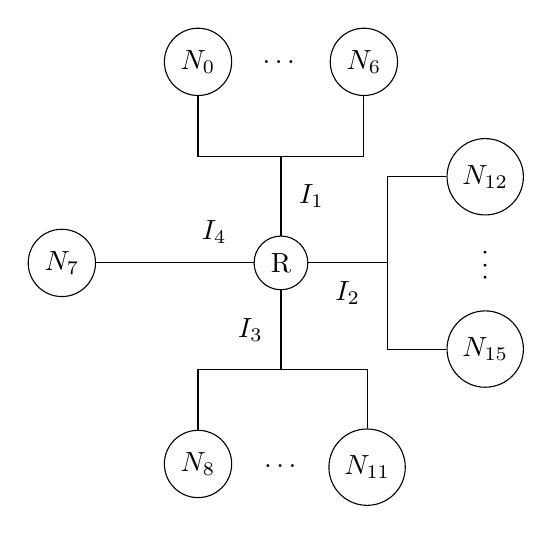
\begin{tikzpicture}[every node/.style={circle, draw}]
  \label{page:network:star}
  \node (r) {R};

  \node [above left=2cm and 0.5cm of r] (n0) {$N_0$}; 
  \node [above right=2cm and 0.5cm of r] (n6) {$N_6$}; 
  \node [draw=none] at ($(n0)!0.5!(n6)$) {\dots}; 
  \coordinate (i1) at ($(r.north)+(0,1)$);
  \draw (r) to node[right, draw=none] {$I_1$} (i1); 
  \draw (n0) |- (i1) -| (n6); 

  
  \node [above right=0.5cm and 2cm of r] (n12) {$N_{12}$}; 
  \node [below right=0.5cm and 2cm of r] (n15) {$N_{15}$};  
  \node [draw=none,rotate=90] at ($(n12)!0.5!(n15)$) {\dots}; 
  \coordinate (i2) at ($(r.east)+(1,0)$);
  \draw (r) to node[below, draw=none] {$I_2$} (i2); 
  \draw (n12) -| (i2) |- (n15); 
  
  \node [below left=2cm and 0.5cm of r] (n8) {$N_8$}; 
  \node [below right=2cm and 0.5cm of r] (n11) {$N_{11}$}; 
  \node [draw=none] at ($(n8)!0.5!(n11)$) {\dots}; 
  \coordinate (i3) at ($(r.south)+(0,-1)$);
  \draw (r) to node[left, draw=none] {$I_3$} (i3); 
  \draw (n8) |- (i3) -| (n11); 
  
  \node [left=2cm of r] (n7) {$N_7$};
  \coordinate (i4) at ($(r.west)+(-1,0)$);
  \draw (r) to node[above, draw=none] {$I_4$} (i4); 
  \draw (n7) -- (i4); 

  
\end{tikzpicture}

% \begin{tikzpicture}[every node/.style={circle, draw}]
%   \label{page:network:star}
%   \node (r) {R};

%   \node [above left=2cm and 0.5cm of r] (n0) {$N_0$}; 
%   \node [above right=2cm and 0.5cm of r] (n6) {$N_6$}; 
%   \node [draw=none] at ($(n0)!0.5!(n6)$) {\dots}; 
%   \coordinate (i1) at ($(r.north)+(0,1)$);
%   \draw (r) to node[right, draw=none] {$I_1$} (i1); 
%   \draw (n0) |- (i1) -| (n6); 

  
%   \node [above right=0.5cm and 2cm of r] (n12) {$N_{12}$}; 
%   \node [below right=0.5cm and 2cm of r] (n15) {$N_{15}$};  
%   \node [draw=none,rotate=90] at ($(n12)!0.5!(n15)$) {\dots}; 
%   \coordinate (i2) at ($(r.east)+(1,0)$);
%   \draw (r) to node[below, draw=none] {$I_2$} (i2); 
%   \draw (n12) -| (i2) |- (n15); 
  
%   \node [below left=2cm and 0.5cm of r] (n8) {$N_8$}; 
%   \node [below right=2cm and 0.5cm of r] (n11) {$N_{11}$}; 
%   \node [draw=none] at ($(n8)!0.5!(n11)$) {\dots}; 
%   \coordinate (i3) at ($(r.south)+(0,-1)$);
%   \draw (r) to node[left, draw=none] {$I_3$} (i3); 
%   \draw (n8) |- (i3) -| (n11); 
  
%   \node [left=2cm of r] (n7) {$N_7$};
%   \coordinate (i4) at ($(r.west)+(-1,0)$);
%   \draw (r) to node[above, draw=none] {$I_4$} (i4); 
%   \draw (n7) -- (i4); 

  
% \end{tikzpicture}

% routing tree
\begin{tikzpicture}[level distance=1cm,
  level 1/.style={sibling distance=6cm},
  level 2/.style={sibling distance=5cm},
  level 3/.style={sibling distance=3cm},
  level 4/.style={sibling distance=2cm},
  level 4/.style={sibling distance=1cm},
  ]
  \label{page:network:tree}

  \node {}
  child {
    % 0 
    node{}
    child {
      % 00
      node {}
      child {
        % 000
        node {$I_1$}
        edge from parent node [above left] {0}
      }
      child {
        % 001
        node {}
        child {
          % 0010
          node {$I_1$}
          edge from parent node [above left] {0}
        }
        child {
          % 0011
          node {}
          child {
            % 00110
          node {$I_1$}
          edge from parent node [above left] {0}
          }
            child {
            %   00111
            node {$I_4$}
            edge from parent node [above right] {1}
          }
          edge from parent node [above right] {1}
        }
        edge from parent node [above right] {1}
      }
      edge from parent node [above left] {0}
    }
    child {
      % 01
      node {}
      child {
        % 010
        node {$I_3$}
        edge from parent node [above left] {0}
      }
      child {
        % 011
        node {$I_2$}
        edge from parent node [above right] {1}
      }
      edge from parent node [above right] {1}
    }
    edge from parent node [above left] {0}
  }
  child {
    % 1
    node{ ? }
    edge from parent node [above right] {1}
  }
  ;
\end{tikzpicture}

\begin{tikzpicture}[every node/.style={circle, draw}]
  \label{page:network:unsorted}
  \node (r) {R};

  % base nodes and interface coordinates: 
  
  \node [above left=2.5cm and 2cm of r] (n0) {$\substack{N_{0}\\ \displayasbinary{0}} $};
  \coordinate (i1) at ($(r.north)+(0,1.75)$);
  \draw (r) to node[right, draw=none] {$I_1$} (i1);   
  \draw (n0) |- (i1); 

  \coordinate (i2) at ($(r.east)+(5,0)$);
  % \node [above right=0.5cm and 5cm of r] (n1) {$\substack{N_{1}\\ \displayasbinary{1}} $};
  \node [above right=0.5cm and 0.5cm of i2] (n1) {$\substack{N_{1}\\ \displayasbinary{1}} $};
  \node [draw=none,rotate=90] at ($(n1)!0.5!(n15)$) {}; 
  \draw (r) to node[below, draw=none] {$I_2$} (i2); 
  \draw (n1) -| (i2); 


  \node [below left=2.5cm and 2.25cm of r] (n4) {$\substack{N_{4}\\ \displayasbinary{4}} $}; 
  \node [draw=none] at ($(n4)!0.5!(n11)$) {}; 
  \coordinate (i3) at ($(r.south)+(0,-1.5)$);
  \draw (r) to node[left, draw=none] {$I_3$} (i3); 
  \draw (n4) |- (i3); 
  
  \node [above left=0.5cm and 5cm of r] (n8) {$\substack{N_{8}\\ \displayasbinary{8}} $};
  \coordinate (i4) at ($(r.west)+(-4,0)$);
  \draw (r) to node[above, draw=none] {$I_4$} (i4); 
  \draw (n8) -| (i4); 

  % ugly, but see the TODO below
  \node [right=of n0] (n2) {$\substack{N_{2}\\ \displayasbinary{2}} $};
  \node [right=of n2] (n5) {$\substack{N_{5}\\ \displayasbinary{5}} $};
  \node [right=of n5] (n9) {$\substack{N_{9}\\ \displayasbinary{9}} $};
  \node [right=of n9] (n14) {$\substack{N_{14}\\ \displayasbinary{14}} $};

  \node [below=of n1] (n3) {$\substack{N_{3}\\ \displayasbinary{3}} $};
  \node [below=of n3] (n6) {$\substack{N_{6}\\ \displayasbinary{6}} $};
  \node [below=of n6] (n10) {$\substack{N_{10}\\ \displayasbinary{10}} $};

  \node [right=of n4] (n7) {$\substack{N_{7}\\ \displayasbinary{7}} $};
  \node [right=of n7] (n11) {$\substack{N_{11}\\ \displayasbinary{11}} $};
  \node [right=of n11] (n12) {$\substack{N_{12}\\ \displayasbinary{12}} $};

  \node [below=of n8] (n13) {$\substack{N_{13}\\ \displayasbinary{13}} $};
  \node [below=of n13] (n15) {$\substack{N_{15}\\ \displayasbinary{15}} $};
  

  
  % TODO: this really should work, but throws errors for prevnode 
  \foreach \startnode/\orientation/\interface/\nodes/\drawstyle/\outdir in {
    0/right/1/{2,5,9,14}/|-/south,
    1/below/2/{3,6,10}/-|/west,
    4/right/3/{7,11,12}/|-/north,
    8/below/4/{13,15}/-|/east,
  } {
    % \foreach \i [remember=\i as \prevnode (initially \startnode)] in \nodes {
    %   \node [\orientation=0.5cm of n\prevnode] (n\i) {$\substack{N_{\i}\\ \displayasbinary{\i}} $};
    % }
    \foreach \i in \nodes {
      \draw (n\i.\outdir) \drawstyle (i\interface); 
    }
  }



\end{tikzpicture}


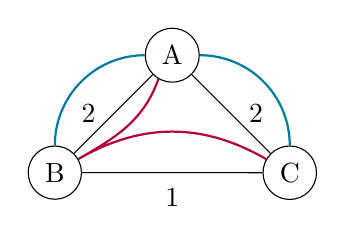
\begin{tikzpicture}[every node/.style={circle}]
  \label{page:routing:shortest_vs_spanning}
  \node [draw] (a) {A};
  \node [draw, below left=of a] (b) {B};
  \node [draw, below right=of a] (c) {C};

  \draw (a) to node [left] {2} (b); 
  \draw (a) to node [right] {2} (c); 
  \draw (b) to node [below] {1} (c); 

  % spanning tree:
  \draw [hpired, thick] (a.240) to[out=250,in=30] (b.30) to[out=30,in=150] (c.150);

  % shortest-path tree:
  \draw [hpiblue, thick] (b.90) to[out=90,in=180] (a)  to[out=0,in=90] (c);
  
\end{tikzpicture}


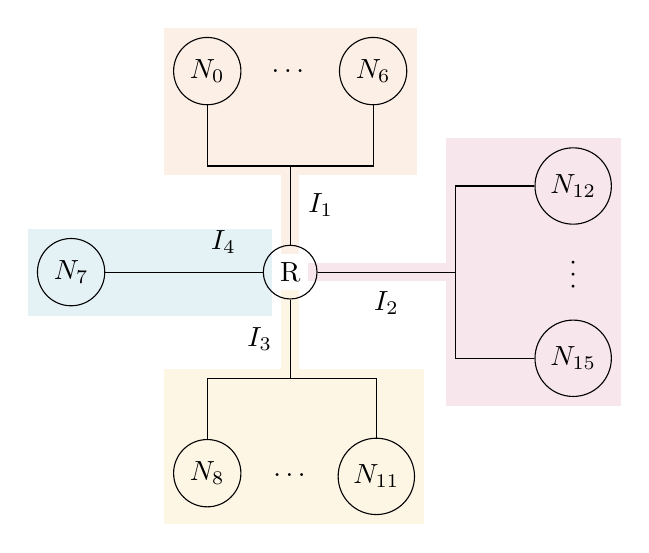
\begin{tikzpicture}[every node/.style={circle, draw}]
  \label{page:network:star:bubbles}
  \node (r) {R};

  \node [above left=2cm and 0.5cm of r] (n0) {$N_0$}; 
  \node [above right=2cm and 0.5cm of r] (n6) {$N_6$}; 
  \node [draw=none] at ($(n0)!0.5!(n6)$) {\dots}; 
  \coordinate (i1) at ($(r.north)+(0,1)$);
  \draw (r) to node[right, draw=none] {$I_1$} (i1); 
  \draw (n0) |- (i1) -| (n6); 

  
  \node [above right=0.5cm and 3cm of r] (n12) {$N_{12}$}; 
  \node [below right=0.5cm and 3cm of r] (n15) {$N_{15}$};  
  \node [draw=none,rotate=90] at ($(n12)!0.5!(n15)$) {\dots}; 
  \coordinate (i2) at ($(r.east)+(1.75,0)$);
  \draw (r) to node[below, draw=none] {$I_2$} (i2); 
  \draw (n12) -| (i2) |- (n15); 
  
  \node [below left=2cm and 0.5cm of r] (n8) {$N_8$}; 
  \node [below right=2cm and 0.5cm of r] (n11) {$N_{11}$}; 
  \node [draw=none] at ($(n8)!0.5!(n11)$) {\dots}; 
  \coordinate (i3) at ($(r.south)+(0,-1)$);
  \draw (r) to node[left, draw=none] {$I_3$} (i3); 
  \draw (n8) |- (i3) -| (n11); 
  
  \node [left=2cm of r] (n7) {$N_7$};
  \coordinate (i4) at ($(r.west)+(-1,0)$);
  \draw (r) to node[above, draw=none] {$I_4$} (i4); 
  \draw (n7) -- (i4); 


  \begin{scope}[on background layer,every node/.style={draw=none,rectangle}]
    % colored bubbles around networks
    \node [fill=hpired!10,fit=(i2)(n12)(n15)] {};
    \node [fill=hpired!10,fit=(i2)(r.east)] {};
    
    \node [fill=hpiorange!10,fit=(i1)(n0)(n6)] {};
    \node [fill=hpiorange!10,fit=(i1)(r.north)] {};

    \node [fill=hpiyellow!10,fit=(i3)(n8)(n11)] {};
    \node [fill=hpiyellow!10,fit=(i3)(r.south)] {};

    \node [fill=hpiblue!10,fit=(i4)(n7)(r.west)] {};
    
  \end{scope}
  
  
\end{tikzpicture}


\end{document} 